\section{Технологический раздел}

\subsection{Архитектура приложения}

\begin{frame}
\begin{center}
	Приложение построено с использованием клиент-серверной архитектуры
	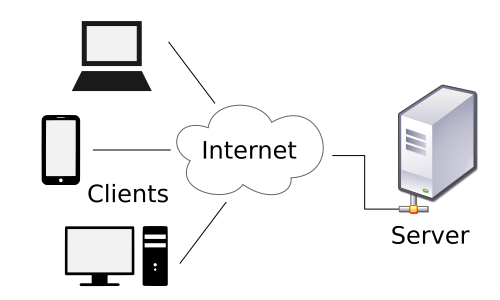
\includegraphics[width=0.6\textwidth]{./Client-server-model.png}
\end{center}
\end{frame}

\subsection{Серверная часть}

\begin{frame}
Инструменты, которые используются непосредственно на сервере.

\begin{itemize}
    \item Go 1.15 --- язык программирования. 
    
    \item Tarantool 2.2.4 --- Резидентная СУБД и сервер приложений.
    
    \item Go-tarantool --- Библиотека для подключения к Tarantool из Go.
    
    \item TarantoolQueue --- Модуль консистентных 
    очередей для Tarantool.

    \item TarantoolDDL --- Модуль декларативного описания таблиц в Tarantool. 
\end{itemize}
\end{frame}

\subsection{Клиентская часть}

\begin{frame}
Инструменты, которые используются в браузере пользователя.
\begin{itemize}
    \item HTML5 --- язык разметки веб-страниц.
    
    \item GoTemplates --- язык шаблонов для HTML страниц. 
    \item CSS --- язык стилей.

    \item Bootstrap --- CSS-фреймфорк.
\end{itemize}
\end{frame}

\subsection{Структура проекта}


\begin{frame}
    \begin{itemize}
        \item Models --- модуль, содержащий реализацию сущностей приложения на языке Go.
        \item Repos --- модуль, содержащий логику доступа к данным
            \item Grant --- модуль доступа к данным привелегий
            \item LabeledTask --- модуль доступа к размеченным данным
            \item Project --- модуль доступа к данным проекта
            \item Schema --- модуль доступа к схемам проектов
            \item Session --- модуль доступа к сессиям пользователей
            \item Task --- модуль доступа к размечаемым данным
            \item User --- модуль доступа к данным пользователей
           \end{itemize}
\end{frame}

\begin{frame}
    \begin{itemize}
        \item Auth ---   модуль, авторизации
        \item Universe --- модуль - глобальный репозиторий, обеспечивающий централизованную работу с подключениями к базе данных
        \item Tarantool --- модуль обеспечивающий загрузку СУБД Tarantool, создание таблиц, загрузку хранимых процедур на Lua.

    \end{itemize}
\end{frame}
